% Chapter 1
\section*{Preface}
In this chapter, we talk about the techniques used in our work to establish mechanism of a working battery. 
\pagebreak
\chapter{Techniques for characterisation} % Main chapter title
\label{chap2} % For referencing the chapter elsewhere, use \ref{Chapter1} 
Performance of a cell cannot be evaluated without two techniques: galvanostatic charge/discharge cycle and cyclic voltammetry. A charge/discharge cycle displays the specific capacity of a material. CV scans help in understanding the voltage profile of a cell.
After continuous charge/discharge cycles, a cathode material undergoes structural changes. To study these changes, we need a few analytical tools. 

\begin{itemize}
    \item Changes in the crystal lattice of a material can be studied in its XRD patterns 
    \item Changes in the oxidation state of an element can be noticed in its XPS spectra
    \item Changes in the vibrational mode of a molecule can be observed in its Raman spectra 
\end{itemize}

\section{X-ray diffraction Studies}
Diffraction of x-rays by crystal planes allows us to derive lattice spacings by using the Bragg's law. 

 \begin{equation} \label{eq1}
     2d\sin\theta \text= n{\lambda}
 \end{equation}
 where d = spacing between diffracting planes,\\
$\theta$ = incident angle,\\ 
n = any integer, and \\
$\lambda$ = wavelength of the incident beam. X-rays produce the diffraction pattern because their wavelength $\lambda$ is typically the same order of magnitude (1-100 $\AA$ ) as the d-spacing between the crystal planes. According to Eq.\ref{eq1} any decrease in 2$\theta$ suggests an increase in the d-spacing. 
A pure crystalline sample such as \ce{MoS2} (Figure \ref{Figures/chap2fig:XRD}a) yields sharp peaks in a XRD pattern since it has a long ordered structure. Random orientation of the powdered material is attained after scanning the sample through a range of 2$\theta$ angles. Conversion of the diffraction peaks to d-spacings allows identification of the sample because each sample has a set of unique d-spacings. Typically, d-spacings of the sample are compared with standard reference patterns (ICDD or JCPDS). For determination of unit cell parameters, each reflection must imply a specific lattice plane indicated by miller indices \textit{hkl} (labelled in red). Structure of activated carbon is much less ordered than graphite. Its pattern shows line broadening of the major diffraction bands, which exist at $\sim$ 25 \textdegree and $\sim$ 44 \textdegree .
%X-ray diffraction shows line broadening of only the principal graphite diffraction bands. This broadening is usually interpreted in terms of dimensions of a hypothetical crystallite. Although the crystallite concept has been used when comparing structures in carbons, it has to be stressed that the crystallite does not exist as such within these structures. The disorganized carbon are present in cross-linkage structures [15] forming non-crystallite structures to form microstructures! 
The Panalytical X-Ray diffractometer was used to record the XRD patterns using Cu-K$\alpha$ radiation at an operating voltage of 45 kV and a 40 mA current. The patterns were run with copper radiation ($\lambda$ =1.5405\AA) at a scanning speed of 2\textdegree in 20 minutes. 

\begin{figure}[tbh!]
\centering
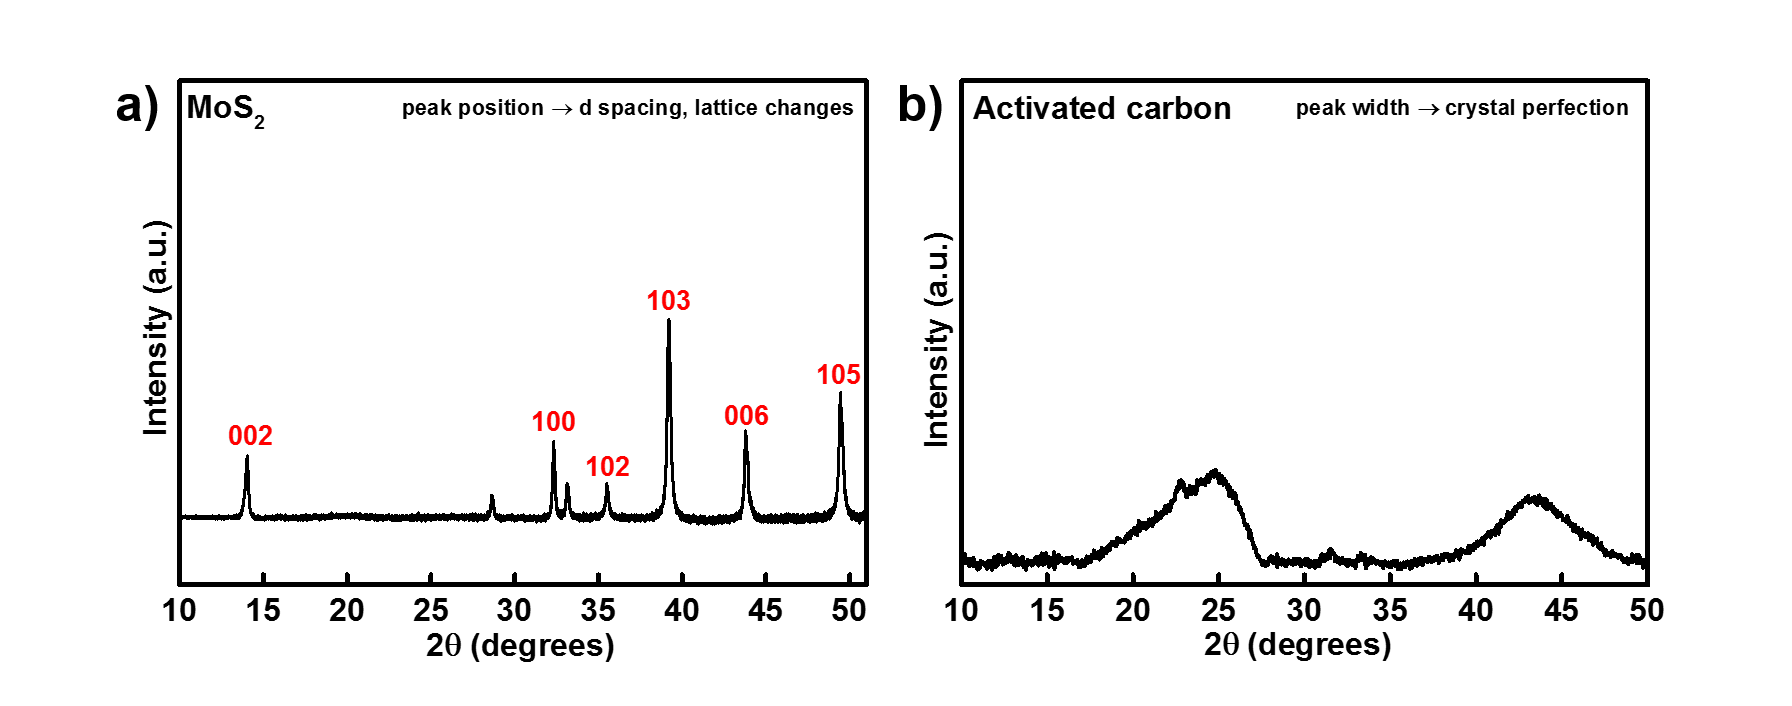
\includegraphics[width=\textwidth]{Figures/chap2fig/XRD}
\caption{XRD pattern of a) bulk molybdenum disulfide and b) activated carbon.}
\label{Figures/chap2fig:XRD}
\end{figure}

\section*{Sample preparation}
The cell was disassembled inside a glove box to prevent the cathode from any contact with air or moisture. The cathode was taken out and washed with dry ethanol to get rid of any remaining electrolyte residue. Since the loading of active material was very low ($\sim$2 mg), the entire electrode (active material coated on molybdenum foil) was mounted on the sample holder for analysis. 

\section{Raman spectroscopy}
Raman spectroscopy is a technique, which is used to determine vibrational modes of a molecule. A source of monochromatic light, usually from a laser, interacts with molecular vibrations in the system, resulting in the energy of the laser photons being shifted up (blue shift) or down (red shift). The shift in energy gives information about any changes taking place in the vibrational modes of a material. 
%This technique uses the inelastic scattering of photons, also known as Raman scattering. 
\begin{figure}[tbh!]
\centering
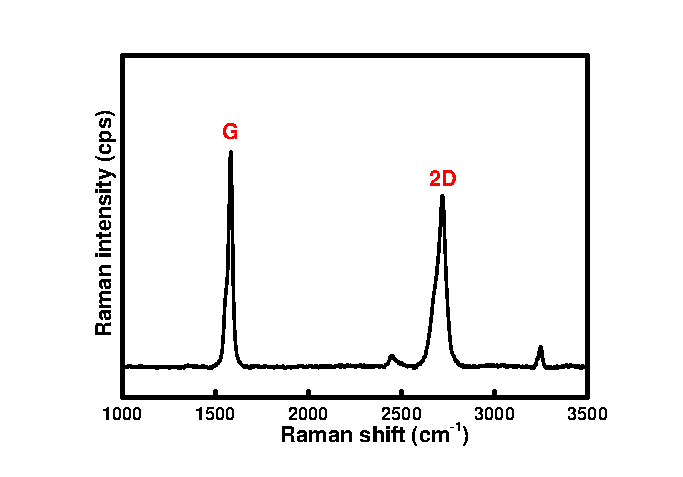
\includegraphics[width=\textwidth]{Figures/chap2fig/Raman}
\caption{XRD pattern of bulk molybdenum disulfide.}
\label{Figures/chap2fig:Raman}
\end{figure}

%Flat and spinner stage?

\section{X-ray photoelectron spectroscopy}
 X-ray photoelectron spectroscopy is used to measure elemental composition and oxidation states of various elements. It is a surface-based technique that quantitatively analyses a sample. By irradiating a sample with a beam of X-rays, kinetic energy and number of electrons escaping from the top 10 nm of the sample are measured. 
%The instrument requires high vacuum (10$^{-8}$ millibar) conditions to count these electrons. The electron emission after irradiation is also called a 'photoelectron effect'. These electrons are separated according to their energies and counted. ,
A normal XPS spectrum is a plot of the number of electrons detected versus the binding energy of the electrons detected. The set of XPS peaks produced at certain binding energies values helps in identifying all the elements, and their chemical environment, that exist in the sample. 
In practice, XPS detects all elements from lithium and above. It cannot easily detect hydrogen or helium because helium has a very small cross-sectional area for photoemission and hydrogen only has one electron which is used in making bonds with  small photoelectron cross-section. Detection limits for most of the elements are in the parts per thousand range. XPS is used to study redox processes taking place in a cell. For example, in Al/\ce{MoSe2} cells, molybdenum oxidised from \ce{Mo^{+4}} to \ce{Mo^{5+}} when the cells charged. 

\begin{figure}[tbh!]
\centering
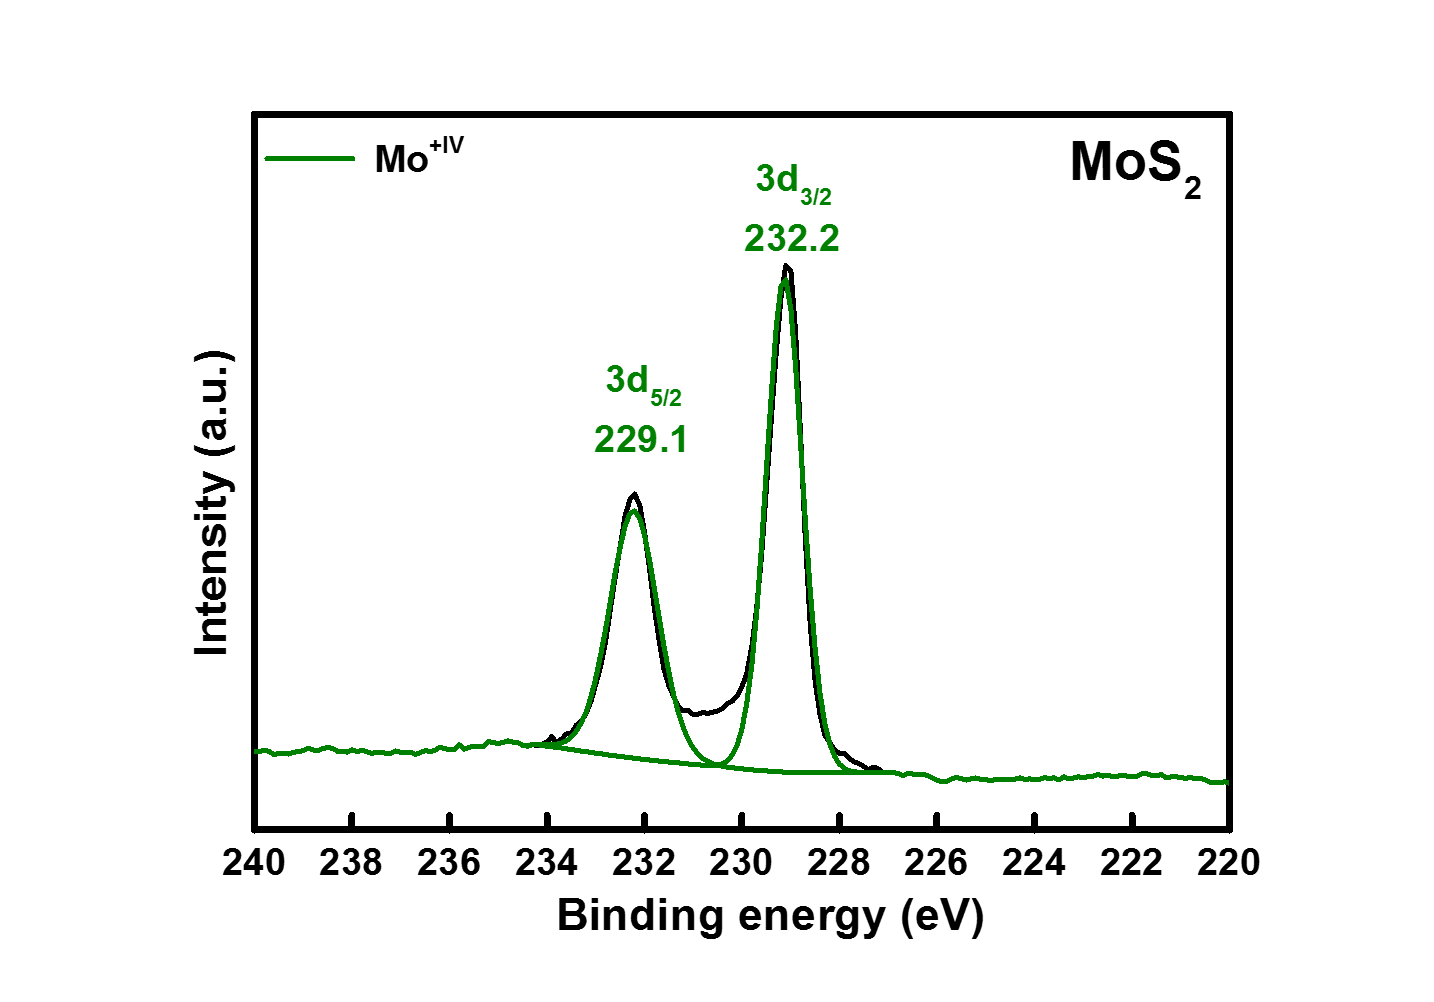
\includegraphics[width=\textwidth]{Figures/chap2fig/XPS}
\caption{XRD pattern of bulk molybdenum disulfide.}
\label{Figures/chap2fig:XPS}
\end{figure}

\section{Cyclic voltammetry}
Cyclic voltammetry (CV) is a technique which measures the current that develops in an electrochemical cell during oxidation and reduction of an analyte (say M). It is performed by cycling the potential of a working electrode, and measuring the resulting current. In Figure \ref{Figures/chap2fig:CV}, we started a forward sweep with a positive scan (lower potential to higher potential). S1 is called a switch potential where the voltage is sufficient enough to cause an oxidation or reduction, and the scan is reversed. Potential is then swept negatively (higher potential to lower potential) until it reaches S2 (another switch potential). In an ideal situation, during forward sweep, M is depleted from the solution as it gets oxidised to \ce{M+}. Further oxidation after scanning higher potentials, leads to growth of a diffusion layer (solution containing M/\ce{M+} ions) at the electrode surface throughout the scan. The layer continues to expand until a certain point, recording maximum current density. However, since diffusion layer continues to grow at this stage, flux of M from the bulk solution to electrode surface decreases. Therefore, current starts to decrease and we get an oxidation peak. A reverse scan converts \ce{M+} back to M (reduction) via similar pathway- formation of a diffusion layer containing M and eventually we record a reduction peak. The two peaks are separated due to the diffusion of the analyte to and from the electrode. If the reduction process is chemically and electrochemically reversible, a peak-to-peak separation of 57 mV is observed \cite{bard_electrochemical_1980}. When there is a high barrier to electrochemical irreversibility, electron transfer reactions are sluggish and more positive/negative potentials are required to observe oxidation/reduction reactions respectively. 

\begin{figure}[tbh!]
\centering
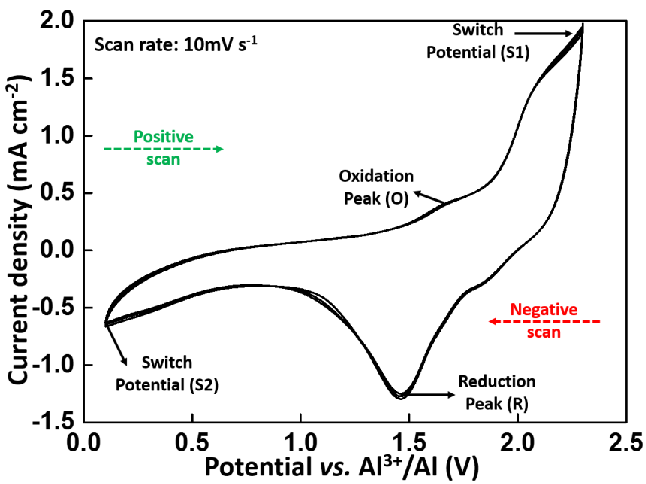
\includegraphics[width=\textwidth]{Figures/chap2fig/CV}
\caption{Cyclic voltammogram of an AIB at a scan rate of 10 mV s$^{-1}$ using a two-electrode cell with aluminium foil acting as a counter and reference electrode.}
\label{Figures/chap2fig:CV}
\end{figure}

Scan rates play a very important role too. If a CV is run on a slower scan rate (0.05 mV s$^{-1}$), diffusion layer grows farther from the electrode, which reduces the flux, consequently decreasing the current value. At a faster scan rate lead (1 V s$^{-1}$), the size of the diffusion layer decreases and higher currents are recorded. Cyclic voltammetry is a helpful tool in understanding the presence of a surface reaction and its reversibility during cell cycles. It can be used for both single-electron and multi-electron processes.  

\section{Galvanostatic charge/discharge cycles}
Galvanostatic  charge and discharge is a method to evaluate the amount of charge stored in a cell typically under constant current. The technique measures voltage at a controlled or fixed current rate. Since the current is repeatedly reversed, it is also known as 'cyclic chronopotentiometry'. It is generally used to estimate their specific capacities and cycling stability of a cell. The total quantity of electricity per mass available from a fully charged cell can be calculated, from the charge transferred during discharge in terms of mAh g$^{-1}$. Specific discharge capacity is frequently measured at different discharging rates to establish rate capability of a cell \cite{pyun_electrochemistry_2012-1}. The voltage profile obtained can be used to identify multi-step redox reactions, in Figure \ref{Figures/chap2fig:ChrononCDC}. 

\begin{figure}[tbh!]
\centering
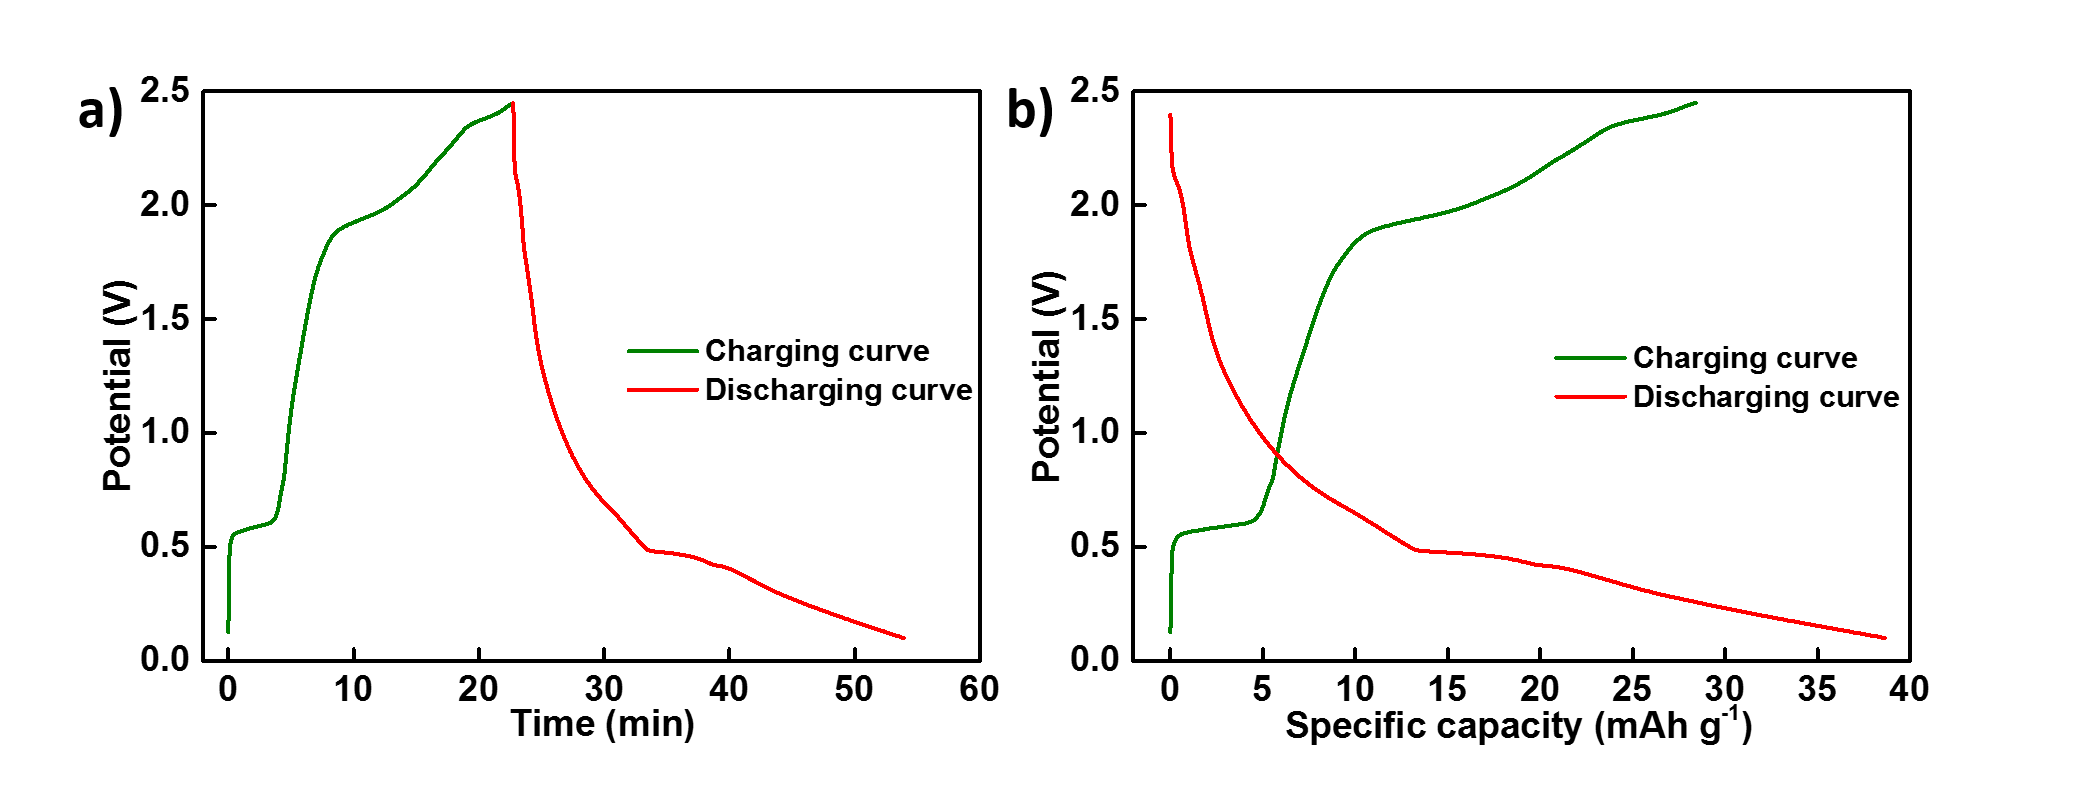
\includegraphics[width=\textwidth]{Figures/chap2fig/ChrononCDC}
\caption{a) Chronopotentiogram- a graph of electric potential versus time, at constant current. b) A galvanostatic charge/discharge curve showing the voltage plateaus at which reactions occur and the charging/discharging capacity.}
\label{Figures/chap2fig:ChrononCDC}
\end{figure}
